\chapter{Gas Processes}
\label{chapter:gas_processes}

There are a lot of very useful and important things that can be done
with gases. Burning gases in an internal combustion engine can power a
car.  Boiling water (and its vapor) can turn a turbine in an
electrical power generation plant. Expanding lungs enable your body to
draw in air and extract oxygen to enable you to live.  Vaporization
and expansion/compression of methylene chloride and water allows a
dunking bird to bob up and down indefinitely over your glass of water
in your dorm room.  Numerous gas processes in the atmosphere drive the
weather system on the Earth.  Expanding and contracting gaseous
bladders enable fish to swim without sinking or floating to the
surface.  Adiabatic heating of a collapsing cloud of hydrogen in space
provides the spark that triggers nuclear fusion and enables the birth
of stars (including our Sun). Hot gases shooting out of an engine can
power an airplane or a rocket.  And many chemical reactions produce
gases that do work on systems (e.g., inflating airbags, firing
ammunition, \dots).

These are just a small sample of the ways in which thermodynamic
processes play a critical role in practical applications and in the
basic functioning of the universe as we know it.  In all of these
cases, it is critical to understand several things: (1) how much work
is required to perform the process or, alternately, how much work is
produced by the process; (2) how much energy in the form of heat must
be added to the gas (or released from the gas) during the process; and
(3) how the thermal energy of the gas either increases or decreases
during the process.  From this perspective, by far the most important
mathematical relation required for analyzing gas processes is one that
we have already seen: the First Law of Thermodynamics
(Eq.~\ref{eq:firstlaw})

\begin{center}
% \boxittext{$\Delta E_\text{therm} = Q_\text{in} + W_\text{on}$}. 
$\Delta E_\text{therm} = Q_\text{in} + W_\text{on}$. 
\end{center}

In this chapter, we will discuss in detail how we can calculate the work, heat and thermal energy changes that occur in thermodynamic processes.

\section{$p$-$V$ diagrams}

An important tool used in analysis of thermodynamics processes is a
plot of pressure versus the volume of a gas, referred to in short as a
{\em $p$-$V$ diagram}. These diagrams are very useful first because
they are directly related to the work done on or by a gas and second
because they are convenient for showing the time evolution of a
thermodynamic process, particularly {\em cyclic} processes that repeat
over and over again, as is the case with many engineering systems.

Given a fixed amount of a gas, a point on a $p$-$V$ diagram represents the
state of the system.  A changing volume and/or pressure results in a
curve on a $p$-$V$ diagram.  Figure \ref{fig:PVdiagrams} shows a few
different processes.  Figure \ref{fig:PVdiagrams}(a) shows a constant
pressure process, with an arrow that indicates an increasing volume
(expansion).  If the arrow were turned around, the same graph would
show a constant pressure compression. In the literature, you may see a
constant pressure process referred to as an {\em isobaric} process
(``iso'' meaning ``same'' and ``baric'' meaning ``pressure'').  Figure
\ref{fig:PVdiagrams}(b) shows a constant volume process, with an arrow
that indicates an increasing volume.

\begin{figure}
\begin{center}
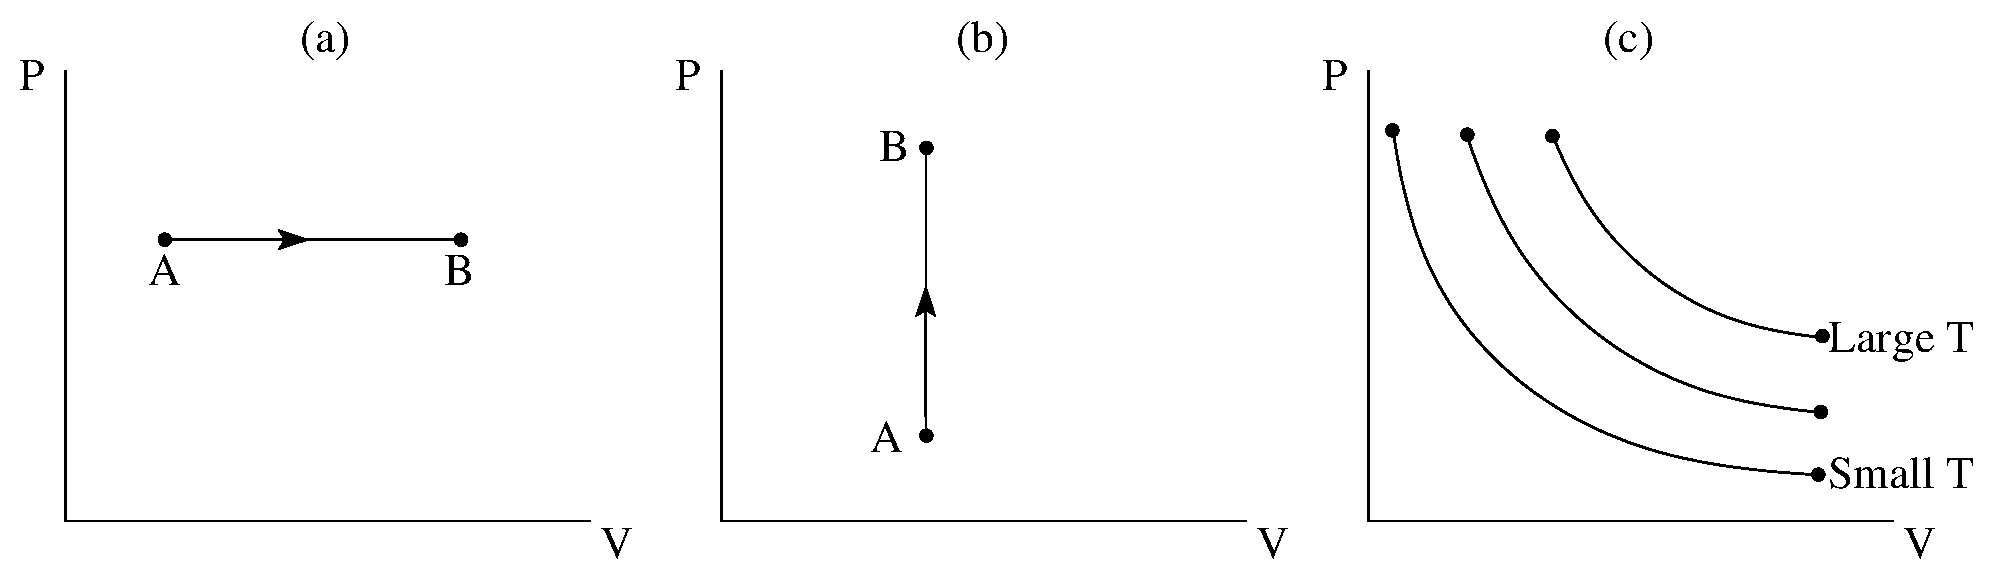
\includegraphics[width=5.0in]{gas_processes/PVdiagrams.eps}
\caption{Processes on a $p$-$V$ diagram.  (a) Constant pressure expansion.
(b) Constant volume process. (c) Three constant temperature (isothermal)
processes.}
\label{fig:PVdiagrams}
\end{center}
\end{figure}

Figure \ref{fig:PVdiagrams}(c) shows a few constant temperature ({\em
  isothermal}) processes. Assuming the number of moles of the gas
doesn't change during a process, the ideal gas law can be used to
determine the relationship between the pressure $p$ and volume $V$ for
an isothermal process: $pV = nRT$ implies $p = nRT/V$.  The result is
a swoopy curve (yes, ``swoopy'' is a valid scientific expression)
since the pressure depends inversely on the volume if $n$ and $T$ are
constant. The resulting curve on a $p$-$V$ diagram is referred to as
an ``isotherm'' and the same graph can show several different
isotherms, depending on the magnitude of the temperature.  Figure
\ref{fig:PVdiagrams}(c) shows that the isotherms corresponding to
higher temperatures are higher and to the right on a $p$-$V$
diagram. It can also be seen that either a constant volume increase in
pressure or an isobaric expansion result in a larger temperature
(indicated by moving to a hotter isotherm).  These results, of course,
are both consistent with the ideal gas law.

\begin{example}{Sketching $p$-$V$ diagrams.}
A gas in a cylinder starts at a temperature $T_1 = 300$ K, volume 
$V_1 = 3.0$ L and pressure $p_1 = 100$ kPa. It
is expanded at constant pressure to twice its initial volume. It is then
compressed isothermally back to the original volume, after which
it is cooled down to a temperature which is half of the initial temperature.
Sketch a $p$-$V$ diagram for the all three processes.

{\bf Solution:} 
\begin{figure}
\begin{center}
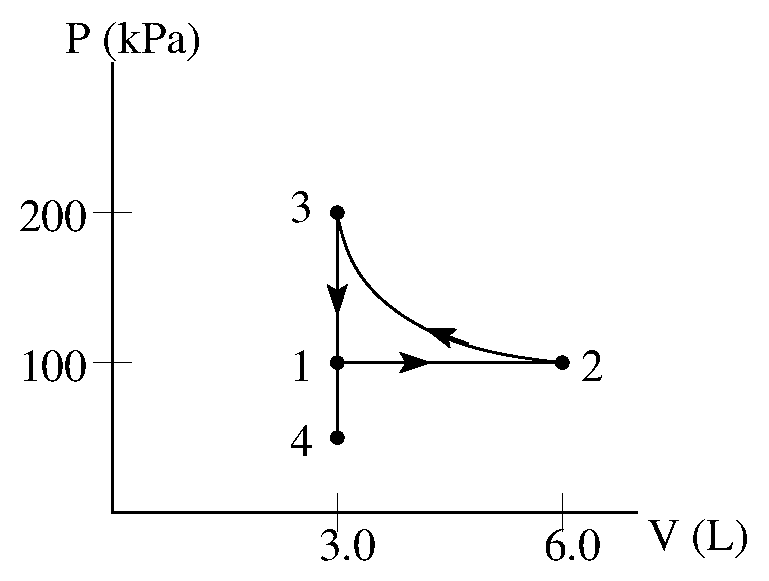
\includegraphics[width=2.0in]{gas_processes/PVexample.eps}
\caption{Solution for Example \ref{ex:PVexample}. Constant pressure
  expansion (1 $\rightarrow$ 2) to twice the initial volume, followed
  by isothermal compression (2 $\rightarrow$ 3) back to initial
  volume, followed by cooling at constant volume (3 $\rightarrow$ 4)
  to temperature half of the initial value.}
\label{fig:PVexample}
\end{center}
\end{figure}
See Fig.~\ref{fig:PVexample}. The constant
pressure expansion (1 $\rightarrow$ 2) also results in a temperature
increase.  Since $pV = nRT$, a doubling of the volume (to 6.0 kPa) at constant
pressure results in a doubling of the temperature (to $600$ K) as well.  So,
after the isothermal compression (2 $\rightarrow$ 3), the gas
is at twice its initial temperature and therefore twice the
initial pressure; i.e., $p_3 = 200$ kPa.  (You could also easily determine
the pressure $p_3$ by noting that with $n$ and $T$ both constant, 
$p_2V_2 = p_3V_3$.) The final process 
(3 $\rightarrow$ 4) brings the gas to a temperature
half of its initial value, and since the final volume is the same
as the initial volume, the final pressure must by half of the initial
pressure; i.e., $p_4 = 50$ kPa.
\label{ex:PVexample}
\end{example}


\section{Calculating work done in gas processes}
\label{section:CalcWork}

Okay, we now have the tools to enable us to calculate the work done on
or by a gas during a process.  The key is the volume.  It turns out that
an expanding gas does work on its environment, whereas it is necessary
for an external agent to do work {\bf on} a gas for it to be compressed.
This can be understood qualitatively by considering a balloon.  If you
want to compress the gas on a balloon, you have to squeeze the balloon,
doing work on the gas.  But if you stick a pin in the balloon, it will pop
and do work on the environment, as evidenced both by the loud ``POP!''
sound and the pieces of balloon fabric that go flying all over the place
after the explosion.

Quantitatively, the work done in an expansion or compression process can
be analyzed as a $p$-$V$ process. For simplicity, let's consider a cylinder
with a fitted piston with mass $m$ that seals in the gas but which can
slide up and down without friction (Fig.~\ref{fig:cylinder}).

\begin{figure}
\begin{center}
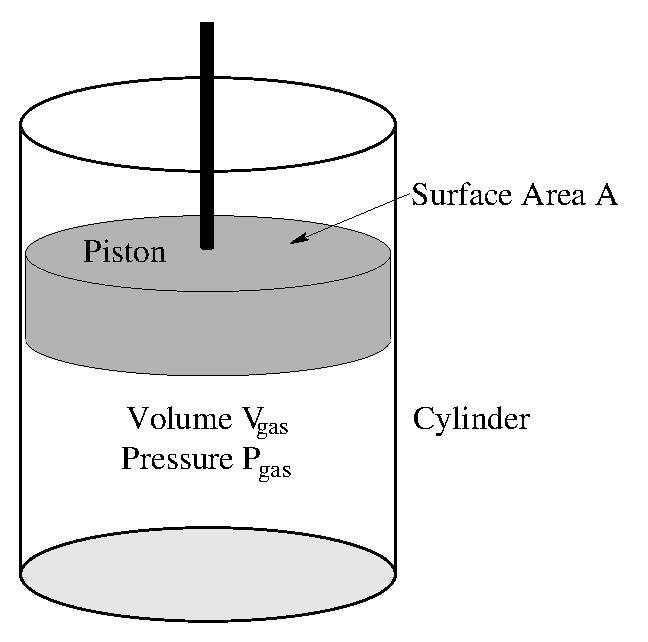
\includegraphics[width=2.0in]{gas_processes/cylinder.eps}
\caption{Piston with surface area $A$ in a cylinder containing
a gas with volume $V_\text{gas}$ and $p_\text{gas}$.}
\label{fig:cylinder}
\end{center}
\label{fig:cylinder}
\end{figure}

The work done on the piston by the gas inside the
cylinder\footnote{Note of course that the gas in the cylinder isn't the only
  thing doing work on the piston in this example: gravity also does
  work, as does the gas {\em outside} the cylinder, along with any
  friction or air resistance.}  can be calculated from the standard
relation for the work done by a spatially-varying force:
$W_\text{by}=\int_{x_i}^{x_f}{F_\text{gas}\,dx}$.  Since the pressure $p$ is the
force divided by the surface area, $F_\text{gas} = p_\text{gas}A$
where $A$ is the cross-sectional area of the piston.  Consequently,
$W_\text{by} = \int_{x_i}^{x_f}{pA\,dx} = \int_{V_i}^{V_f}{p\,dV}$ where we are dropping the
``gas'' subscripts. This result deserves its own line and an equation
number:
\begin{equation}
W_\text{by} = \int_{V_i}^{V_f} p\,dV
\label{eq:WorkBy}
\end{equation}
So, the work done by the gas is simply the integral of the pressure,
integrated over the volume.  And the work done {\em on} a gas is just the
opposite:  
\begin{equation}
W_\text{on} = -\int_{V_i}^{V_f} p\,dV
\label{eq:WorkOn}
\end{equation}
Note also that we can also calculate the work
by determining the area under a curve of $p$ versus $V$, i.e., the area in a
$p$-$V$ diagram.  Here is another example of how useful $p$-$V$ diagrams can be,
since they display quite directly the work done on or by a gas process.


{\bf NOTE:} the sign of the work is critically important.  There is a big
difference between a positive and a negative value, e.g., the work
done by a process $W_\text{by}$. For a car engine, a positive
value of $W_\text{by}$ means that the car is able to drive, whereas a negative
value for $W_\text{by}$ means that you have to push the car to get it to go.

Special cases:

\begin{itemize}
\item {\bf Constant volume processes}.  If the volume remains constant during a
process, the work done on and by the gas is zero.

\item {\bf Isobaric (constant pressure) processes}. In this case, the
  work done by the gas is
\begin{equation}
W_\text{by} = \int_{V_i}^{V_f}p\,dV = p\int_{V_i}^{V_f}\,dV = p\Delta V.
\end{equation}
So, the work done {\bf on} the gas $W_\text{on} = -W_\text{by} =
-p\Delta V$.  This can also been seen easily from a $p$-$V$ diagram
for an isobaric process (Fig.~\ref{fig:PVdiagrams}a): the area under
the curve is simply the area of the rectangle $p\Delta V$.

\item {\bf Isothermal (constant temperature) processes}. In this case,
  the work done by the gas 
\begin{align}
  W_\text{by} &= \int_{V_i}^{V_f}p\,dV =
  \int_{V_i}^{V_f}\frac{nRT}{V}\,dV = nRT\int_{V_i}^{V_f}\frac{dV}{V} 
= nRT[\ln V]_{V_i}^{V_f}  \nonumber\\
  &= nRT( \ln V_f -\ln V_i)
  = nRT\ln\biggl(\frac{V_f}{V_i}\biggr).
\end{align}
 And, of course, the work done {\bf on} the gas $W_\text{on} =
 -W_\text{by} = -nRT\ln (V_f/V_i)$.

{\bf Useful trick:} note that since the ideal gas law states that $pV = nRT$, the work done by 
a gas during an isothermal process can also be written as $W_\text{by}
= pV\ln (V_f/V_i)$. This is really useful if you know the pressure
and volume at any moment during the isothermal process but don't know
the temperature.

\item {\bf Straight-line processes on a $p$-$V$ diagram}. In these cases, the work
can be determined by determining the area under the curve. 

\item If you can't figure it out from any of the four approaches, there is
one other way in which you will be able to calculate the work done on
or by a gas during a processes: use the First Law of Thermodynamics.
If you have a process where you can determine the heat flowing in $Q_\text{in}$
and the change in the thermal energy $\Delta E_\text{therm}$, then you will be able
to find $W_\text{on} = \Delta E_\text{therm} - Q_\text{in}$.

\end{itemize}

Remember that the sign of the work depends on whether the volume is
increasing or decreasing. If $V$ increase, $W_\text{by}$ is positive
and $W_\text{on}$ is negative, and if $V$ decreases, then
$W_\text{by}$ is negative and $W_\text{on}$ is positive.

{\bf A note about units:} in standard units, if pressure is in N/m$^2$
(i.e., Pa) and volume is in m$^3$, the resulting calculated work wil
be in J.  But in many realistic problems, the pressure is given in kPa
and the volume is given in L.  Since $1\units{L} = 10^{-3}
\units{m$^3$}$ and 1 kPa = $10^3$ Pa, a calculation of work using L
and kPa also gives an answer in J. So, it isn't necessary to convert
to Pa and m$^3$ when doing these calculations.


\begin{example}{Calculating work for gas processes}
Calculate the work done on the gas for each of the three processes in
Example \ref{ex:PVexample} (see Fig.~\ref{fig:PVexample}).

{\bf Solution:} Let's deal with each of the three processes in turn:
\begin{itemize}
\item {\bf Process $1 \rightarrow 2$:} This is a constant pressure
  expansion.  First, we need to recognize that since the volume is
  increasing, the work done {\bf by} the gas $W_\text{by}$ is
  positive, so $W_\text{on}$ is negative.  We can figure this out
  easily enough by recognizing that $W_\text{by}$ is simply the area
  under the curve
\begin{equation}
W_\text{by} = \int_{V_1}^{V_2}p\,dV= (100\units{kPa})(6.0\units{L} -
3.0\units{L}) = 300\units{J}. \end{equation}

Alternately, this could also be determined by $W_\text{by} =
\int_{V_1}^{V_2}p\,dV = p\Delta V$ (since this is a constant pressure
process), giving
\begin{equation}
 W_\text{by} = 
(100\units{kPa})(6.0\units{L} - 3.0\units{L}) = 300\units{J}.
\end{equation}
So, $W_\text{on} = -W_\text{by} = -300$ J.

\item {\bf Process $2 \rightarrow 3$:} This is an isothermal
  compression, so $W_\text{on} = -W_\text{by} = -nRT\ln (V_3/V_2)$. We
  don't know how many moles of gas there are, but we could figure it
  out using the Ideal Gas Law.  {\bf But we aren't going to do that},
  because we can replace $nRT$ with either $p_2V_2$ or $p_3V_3$. So,
\begin{equation}
W_\text{on} = -p_2V_2\ln\biggl(\frac{V_3}{V_2}\biggr) = -(100 \units{kPa})(6.0 L)\ln \biggl(\frac{3.0 L}{6.0 L}\biggr) = 416 \units{J}.
\end{equation}
 Note that this is a positive number, which makes sense
since it is a compression, and we know that $W_\text{on}$ is positive for a
compression.  Note also that the work for the  process $2 \rightarrow 3$ 
has a larger magnitude than that for process $1 \rightarrow 2$, which also
makes sense because there is a larger area under the curve $2 \rightarrow 3$
than under the curve $1 \rightarrow 2$.

\item {\bf Process $3 \rightarrow 4$:} This is a constant volume process,
so $W_\text{on} = 0$. This is also consistent with work as area under the curve,
as there is no area under the process $3 \rightarrow 4$.
\end{itemize}
\end{example}

\section{Adiabatic processes}

In many real gas processes, there is no heat flow either into or out
of the system; i.e., $Q_\text{in} = 0$. This occurs if (a) the system
is completely isolated from its environment so there is no way for
heat to be exchanged with its surroundings (e.g., if it is surrounded
by insulation); or (b) if the processes occurs so rapidly that there
simply isn't enough time for there to be an appreciable flow of heat
into or out of the system.

A process with no heat flow (i.e., $Q_\text{in} = 0$) is referred to as an
{\em adiabatic} process. The calculations of $Q_\text{in}$, $W_\text{on}$ and
$\Delta E_\text{therm}$ are easier for adiabatic processes, predominately because
$Q_\text{in} = 0$ (by definition), so if you can determine one of either
$W_\text{on}$ or $\Delta E_\text{therm}$, you can get the other from the First
Law of Thermodynamics.
Calculating $W_\text{on}$ is non-trivial for an adiabatic process (it isn't
one of the four special cases discussed in the previous section), so
for an adiabatic process, we will typically find $\Delta E_\text{therm}$  first.
We'll discuss how to do that in the next section. 

First, however, we
can quickly get an idea of how an adiabatic process looks on a $p$-$V$
diagram. Since $Q_\text{in} = 0$ for an adiabatic process, the First Law
becomes:  $\Delta E_\text{therm} = W_\text{on}$; i.e., any work done on the system
goes into increasing the thermal energy.  And recall that the thermal
energy of a gas increases with the temperature of the gas.
For an adiabatic compression, $W_\text{on} > 0$
which means that $\Delta E_\text{therm} > 0$.  This means that for any
adiabatic compression, the gas heats up (i.e., the temperature increases).
This makes sense:  we are doing work on the gas to compress it, and that
work goes into heating up the gas and increasing the temperature.

\begin{figure}
\begin{center}
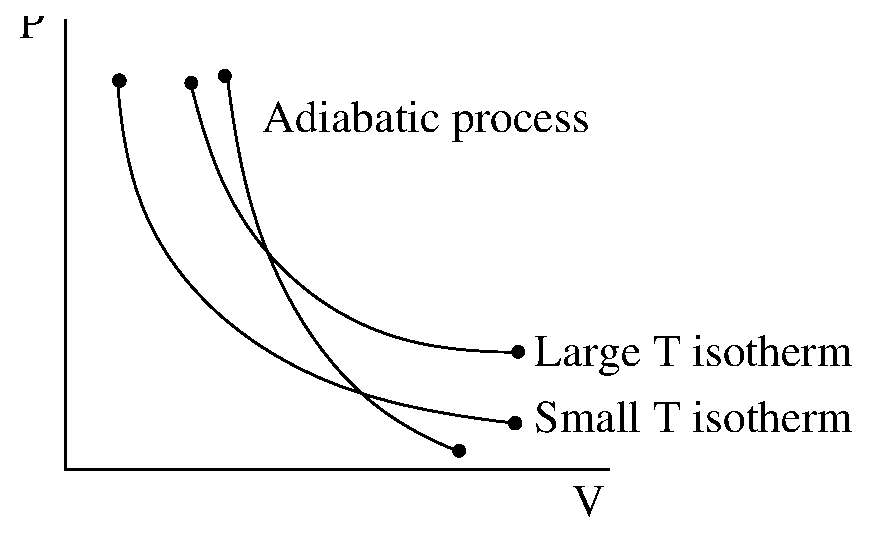
\includegraphics[width=2.0in]{gas_processes/IsothermAdiabats.eps}
\caption{$p$-$V$ diagram showing both isotherms and adiabats.}
\label{fig:IsothermAdiabats}
\end{center}
\end{figure}

Since an adiabatic compression results in an increase in temperature,
the curve on a $p$-$V$ diagram for an adiabatic compression must go to larger
and larger temperature, which means that and adiabatic process is
associated with a curve (an ``adiabat'') that is steeper than those for
isothermal processes (i.e., ``isotherms''). This can be seen in 
Fig.~\ref{fig:IsothermAdiabats},
 which shows curves for both adiabatic and isothermal processes.

To make a quantitative statement about the functional form of the
adiabatic curves, we need to consider the type of gas. 
As discussed in section \ref{section:TheGasState}, the thermal energy
of a gas depends on the type of molecules in that gas.  (See 
Eqs.~\ref{eq:monatomic_ideal_gas}, \ref{eq:diatomic_ideal_gas} and 
\ref{eq:EthermIdealGas}.) In particular, the behavior of the gas depends
on the number of degrees of freedom $f$ and the ``adiabatic exponent''
$\gamma = \frac{f+2}{f}$. (Recall that $\gamma = 5/3$ for a monatomic
gas with 3 degrees of freedom, and $\gamma = 7/5$ for a diatomic
gas with 5 degrees of freedom.) Without going through the full 
derivation,\footnote{The full derivation involves solving 
a differential equation, but differential equations are not required for 
PHYS 211.} an adiabatic process has pressure and volume that are
related via:
\begin{equation}
pV^{\gamma} = (\text{constant}).
\label{eq:PVGamma}
\end{equation}
From a practical perspective, this means that given three of the four quantities
$p_i$, $V_i$, $p_f$ and $V_f$, for an adiabatic process the fourth can be determined from the relation
$p_iV_i^{\gamma} = p_fV_f^{\gamma}$.

Similarly, a relation can be found between the temperature $T$ and volume $V$
during an adiabatic process\footnote{Simply combine Eq.~\ref{eq:PVGamma} with
the Ideal Gas Law.}: $TV^{\gamma - 1} = (\text{constant})$.

\begin{example}{Adiabatic expansion}
A diatomic gas with an initial pressure, temperature and volume of 150 kPa,
300 K and 3.5 L is compressed to a volume of 0.5 L; the compression is
so fast that there isn't enough time for heat to flow into or out
of the gas. Calculate the pressure and temperature of the gas after the
compression.

{\bf Solution:} Since there isn't enough time for heat to flow into or
out of the gas, this is an adiabatic process.  And since the gas is
composed of diatomic molecules at a temperature that isn't too high,
there are 5 degrees of freedom for the gas and $\gamma = \frac{f+2}{f} = 7/5$.
Since this is an adiabatic process, $pV^{\gamma} = $constant, so
so $p_iV_i^\gamma = p_fV_f^\gamma$, which implies
\begin{equation}
 p_f=p_i\biggl(\frac{V_i}{V_f}\biggr)^\gamma
= 150 \units{kPa}\biggl(\frac{3.5 \units{L}}{0.5 \units{L}}\biggr)^{7/5} = 
2290\units{kPa}.
\end{equation}
As for the temperature:  since this is an adiabatic process, $TV^{\gamma - 1}$
= constant, so $T_iV_i^{\gamma - 1} = T_fV_f^{\gamma - 1}$ which implies
\begin{equation}
T_f = T_i\biggl(\frac{V_i}{V_f}\biggr)^{\gamma - 1} = (300 \units{K})\biggl(\frac{3.5 \units{L}}{0.5 \units{L}}\biggr)^{7/5-1} = 653 \units{K}.
\end{equation}  Note that the gas heats up, which is 
always the case for an adiabatic compression.
\end{example}

\section{Calculating heat and thermal energy changes}

Okay, we now have everything that we need to determine 
the heat $Q_\text{in}$, the work $W_\text{on}$ or $W_\text{by}$ and the change in
thermal energy $\Delta E_\text{therm}$ for an arbitrary process. This
will prove to be quite important when we talk about heat engines
in a couple of chapters.

We have already discussed the different approaches that you can use
to determine the work done on or by a gas (see the bulleted list at the
end of Section \ref{section:CalcWork}). We can make similar
bulleted lists for $\Delta E_\text{therm}$ and $W_\text{on}$ or $W_\text{by}$.

To determine the change in the thermal energy for a process:
\begin{itemize}
\item The easiest case is if the process is isothermal or if it
ends up at the same temperature that it started (e.g., if it is a
{\em cyclic} process), then $\Delta E_\text{therm} = 0$. 
\item If you know how many degrees of freedom the gas molecules
have ($f = 3$ or $5$ for monatomic and diatomic gases, respectively,
for example), then $\Delta E_\text{therm} = \frac{f}{2}nR\Delta T$.
This is convenient if you know the starting and ending temperature.

{\bf Useful trick redux:} the same $pV = nRT$ trick can be used here.
If you don't know the initial and final temperatures but you {\bf do} 
know the initial and
final pressure and volume, then $\Delta E_\text{therm} = \frac{f}{2}(p_2V_2
- p_1V_1)$.

\item If neither of the above work, but you can figure out $Q_\text{on}$ and
$W_\text{on}$, then you can get $\Delta E_\text{therm}$ from the first law:  
$\Delta E_\text{therm} = Q_\text{on} + W_\text{on}$.
\end{itemize}

We can make a similar bulleted list for how to determine the heat 
flow $Q_\text{in}$:
\begin{itemize}

\item The easiest case is if the problem states that the process is
adiabatic\footnote{The problem might be subtle about this: it might
say ``... for a well-insulated system ...'' or ''... for a very
rapid process ...,'' either of which imply no heat exchange between
the system and the environment.}: in this case, $Q_\text{in} = 0$.

\item If the process is not adiabatic, then you will be using the first
law of thermodynamics to find $Q_\text{in}$: $Q_\text{in} = \Delta E_\text{therm} - W_\text{on}$.

\end{itemize}

For all of these calculations, {\bf make sure that you check the signs}
of everything.  There is a really big difference between positive and 
negative values for each of $\Delta E_\text{therm}$, $Q_\text{in}$ and
$W_\text{on}$ for a gas process.\footnote{If you ever forget this, set
your car in neutral and push it from here to New York --- that's what
you would have to do for a car whose engine is described by a positive
value of $W_\text{on}$.}


\begin{example}{A complete cycle}
Consider a fixed amount of an ideal gas of diatomic molecules undergoing
the processes shown in Fig.~\ref{fig:CycleExample}.  The gas starts at
point {\bf A} in the diagram and expands along the path {\bf
  A}$\longrightarrow${\bf B} with no heat flowing into or out of the
gas.

(a) Calculate the pressure of the gas at point {\bf B} after the
expansion. (b) Determine the net work done {\bf on} the gas and the heat flow $Q_\text{in}$ 
in one complete cycle 
({\bf A}$\longrightarrow${\bf B}$\longrightarrow${\bf C}
$\longrightarrow{\bf A}$).
\begin{figure}
\begin{center}
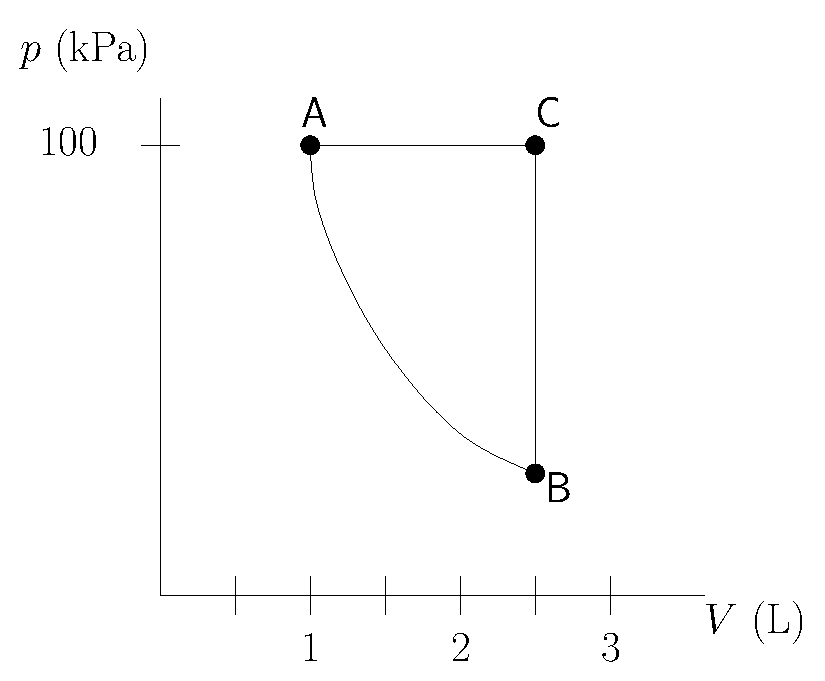
\includegraphics[width=3.0in]{gas_processes/cycle.eps}
\caption{For Example \ref{ex:cycle2010tst3}.}
\label{fig:CycleExample}
\end{center}
\end{figure}
\label{ex:cycle2010tst3}

{\bf Solution:} (a) Since the process $A \rightarrow B$ is adiabatic,
$pV^\gamma$ = constant and $p_AV_A^\gamma = p_BV_B^\gamma$
so
\begin{equation}
  p_B = p_A\biggl(\frac{V_A}{V_B}\biggr)^{7/5} = 100
  \units{kPa} \times \biggl(\frac{1.0 \units{L}}{2.5 \units{L}}\biggr)^{7/5}
  = 27.7 \units{kPa}.
\end{equation}

(b) We will calculate the work done on the gas for each
of the three processes and add up the results to get the net work. 
To figure out the total heat flow $Q_\text{in}$ we could do something similar ---
i.e., calculate $Q_\text{in}$ for each process and then add them up. But there
is an easier way: since we know that $\Delta E_\text{therm} = 0$ for the complete
cycle, once we have determined the total $W_\text{on}$ for the complete
cycle, we can use the First Law of Thermodynamics to get $Q_\text{in}$ for
the complete cycle.

Let's start with {\bf process $A \rightarrow B$}.  This is an adiabatic process,
so $Q_\text{in} = 0$. Calculating work is tricky for adiabatic processes,
so we'll find $\Delta E_\text{therm}$ first and then use the First Law to get
$W_\text{on}$. This is a diatomic gas, so $f = 5$ and $\Delta E_\text{therm} =
\frac{f}{2}nR\Delta T$. We could calculate $T_B$, but we won't bother,
because $\Delta E_\text{therm}$ can be found with the pressures and volumes
given:
\begin{align}
\Delta E_\text{therm} &= \frac{f}{2}(p_BV_B - p_AV_A) = \frac{5}{2}
\Bigl(27.7 \units{kPa} \times 2.5 \units{L} -
100 \units{kPa}\times 1.0 \units{L}\Bigr)
\nonumber\\ &= -76.7 \units{J}.
\end{align}
We can now find the work done on the gas via the First Law:
%$\Delta E_\text{therm} = Q_\text{in} + W_\text{on} \rightarrow
\begin{equation}
  W_\text{on} = \Delta E_\text{therm} - Q_\text{in} =
  -76.7 \units{J} - 0 = -76.7 \units{J}.
\end{equation}

{\bf Process $B \rightarrow C$:} this is a constant volume process, so 
$W_\text{on} = 0$.


{\bf Process $C \rightarrow A$:} this is a constant pressure (isobaric)
process, so
\begin{equation}
  W_\text{on} = -p\Delta V = -p(V_A - V_C) = -100 \units{kPa}(1.0
\units{L} - 2.5 \units{L}) = 150 \units{J}.
\end{equation}

So, the net work $W_\text{on}$ done on the gas for the complete cycle 
$A \rightarrow B \rightarrow C \rightarrow A$ is
\begin{align}
  W_\text{on}^\text{net} &= W_\text{on}^{A\to B}+W_\text{on}^{B\to C}+W_\text{on}^{C\to A}
  \nonumber\\
   &= -76.7 \units{J} + 0\units{J}
+ 150 \units{J} = 73.3 \units{J}.
\end{align}

As for the total heat flow $Q_\text{in}$ for the entire cycle, we can use
the First Law:
%$\Delta E_\text{therm} = Q_\text{in} + W_\text{on} \rightarrow
\begin{equation}
  Q_\text{in} = \Delta E_\text{therm} - W_\text{on} = 0 - 73.3 \units{J}
  = -73.3 \units{J}.
\end{equation}
So, what this
means is that for the entire cycle, 73.3 J of heat flows {\bf out} of
the gas.

\end{example}


\newpage

\section*{Problems}
\markright{PROBLEMS}

\begin{problem} 
 Three identical gas-cylinder systems are compressed from the
 same initial state to final states that have the same volume, one
 isothermally, one adiabatically, and one isobarically. Which
 system has the most work done on it? The least?
\label{prob:ThreeCompress}
\end{problem}

\begin{problem}
The relation between thermal energy and temperature depends on the type
of gas molecule:  for a monatomic gas, $\Delta E_\text{therm} = \frac{3}{2}nR\Delta T$
and for a diatomic gas, $\Delta E_\text{therm} = \frac{5}{2}nR\Delta T$. In your
own words --- and discussing explicitly the microscopic picture of gases ---
explain why it is that you need to put more thermal energy into a diatomic
gas than for a monatomic gas to raise the temperature by 1 K.
\end{problem}

\begin{problem}
Consider a piston in a car engine that is compressing an air-gasoline
mixture before ignition, all in the gas state.  
\begin{enumerate}
\item Under what circumstances would the compression be adiabatic? 
(There are a couple of ways to get an adiabatic compression, one of
which is more relevant to a car engine.)
\item Use the First Law of Thermodynamics to argue that the gas heats
up if the compression is adiabatic.  Where does that additional thermal energy
come from during this process?
\end{enumerate} 
\end{problem}

\begin{problem}
A gas with $n$ moles of molecules starts with a temperature $T_1$,
pressure $p_1$ and volume $V_1$. Draw a $p$-$V$ diagram for the following
multi-step processes (and label each process with its letter a, b, c
or d): 
\begin{enumerate}
\item The gas expands at a constant pressure to twice its initial
volume.
\item The gas is then compressed isothermally back to its initial
volume.
\item The gas then expands adiabatically back to its initial
pressure.
\end{enumerate}
\end{problem}

\begin{problem}
A gas with $n$ moles of molecules starts with a temperature
$T_1$, pressure $p_1$ and volume $V_1$. Draw a $p$-$V$ diagram
for the following multi-step processes:
\begin{enumerate}
\item The gas is heated up at constant volume, doubling its
initial temperature.
\item The gas expands adiabatically until the pressure returns
to $1.5p_1$.
\item A vent is opened, allowing gas to escape until the pressure returns
to the original pressure $p_1$.
\item The gas is compressed isothermally until the volume returns to the
original volume $V_1$.
\end{enumerate}
\end{problem}

\begin{problem}
Calculate the work done on a gas as it undergoes the process shown
in the $p$-$V$ diagram (Fig.~\ref{fig:PVProblem}). 
\begin{figure}
\begin{center}
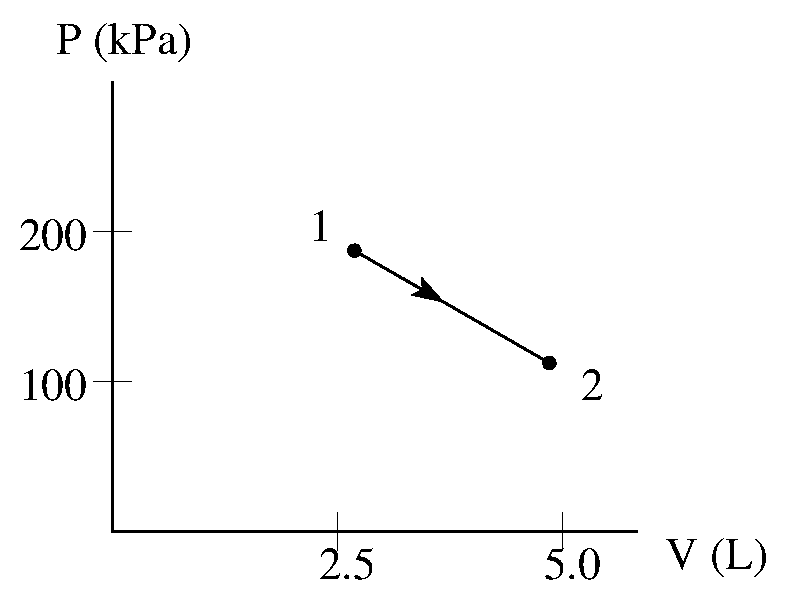
\includegraphics[width=2.5in]{gas_processes/PVProblem.eps}
\caption{For Prob.~\ref{prob:PVProblem}.}
\label{fig:PVProblem}
\end{center}
\label{prob:PVProblem}
\end{figure}

\end{problem}

\begin{problem}
A piston initially contains 1.2 moles of a monatomic gas at a pressure
of 210 kPa and a volume of 0.25 L. The gas expands at constant pressure
to a volume of 0.47 L.  Calculate the work done on the gas during this
process.
\end{problem}

\begin{problem}
A piston initially contains 0.75 moles of a diatomic gas at a pressure
of 105 kPa, a temperature 350 K and a volume of 0.33 L.  The gas
is ignited, raising the temperature rapidly to 550 K without a significant
change in the volume.  Calculate the work done on the gas during this
process.
\end{problem}

\begin{problem}
A monatomic ideal gas undergoes an isothermal compression from an initial
volume of 7.0 L and pressure 100 kPa to a final volume and pressure
of 2.0 L and 350 kPa, respectively. The temperature along the isotherm
is 120$^\circ$ C.
\begin{enumerate}
\item Determine the number of moles of this gas.
\item Determine the work done {\em on the gas} during this process.
\item Determine the heat flowing into the gas during this process.
\end{enumerate}
\end{problem}

\begin{problem}
Consider a fixed amount of an ideal monatomic gas undergoing the
{\em adiabatic} process illustrated in Fig.~\ref{fig:gasProcess2}.
\begin{figure}
\begin{center}
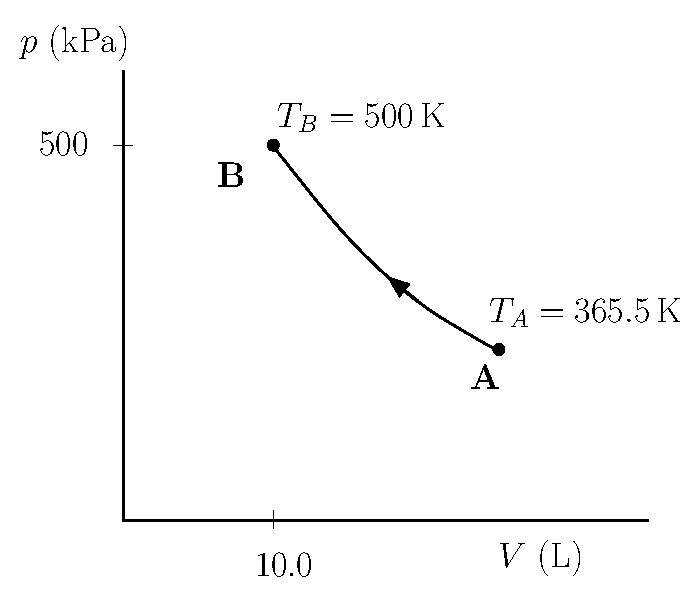
\includegraphics[width=2.0in]{gas_processes/gasProcess2.eps}
\caption{For problem \ref{prob:adiabatic}.}
\label{fig:gasProcess2}
\end{center}
\end{figure}
\begin{enumerate}
\item Calculate the number of moles in the gas.
\item Calculate the work done on the gas between points {\bf A}
and {\bf B}.
\end{enumerate}
\label{prob:adiabatic}
\end{problem}

\begin{problem}
\begin{enumerate}
\item Use the Equipartition Theorem to determine a relation between the
thermal energy change $\Delta E_\text{therm}$ and the temperature
change $\Delta T$ for a monatomic {\em flattium} gas where the
molecules can move only in two dimensions.
\item Do the same thing, but this time for a diatomic flattium gas.
\end{enumerate}
\end{problem}

\begin{problem}
The ``5/2'' in the $\Delta E_\text{therm}$ relation for a diatomic gas (as
opposed to ``3/2'' for a monatomic gas) comes from the fact that
a diatomic molecule can also rotate in two different directions, 
adding two terms to the Equipartition Theorem. But if the gas is
{\em really} hot, it can also excite {\em vibrations} for diatomic
molecules, which provides two more terms in the equation for the energy
of a diatomic molecule: one for the kinetic energy of the vibration and
one for the potential energy of the vibrating molecule. What might you
expect for the relation between $\Delta E_\text{therm}$ and $\Delta T$
for a diatomic gas where the molecules are also vibrating?
\end{problem}

\begin{problem}
A piston contains 0.65 moles of diatomic Nitrogen gas (N$_2$),
with an initial pressure and volume of 110 kPa and 0.15 L, respectively.
The piston compresses the gas adiabatically to a volume 0.062 L.
Calculate the pressure of the gas after this compression.
\end{problem}

\begin{problem}
A piston contains 0.45 moles of monatomic Helium gas, with an initial
volume and temperature of 0.12 L and 285 K, respectively. The
piston expands the gas adiabatically to a volume of 0.31 L.
Calculate the temperature of the gas after this expansion.
\end{problem}

\begin{problem}
A fixed amount of diatomic ideal gas goes through the cycle as shown
in Fig.~\ref{fig:pv_diagram}.
\begin{figure}
\begin{center}
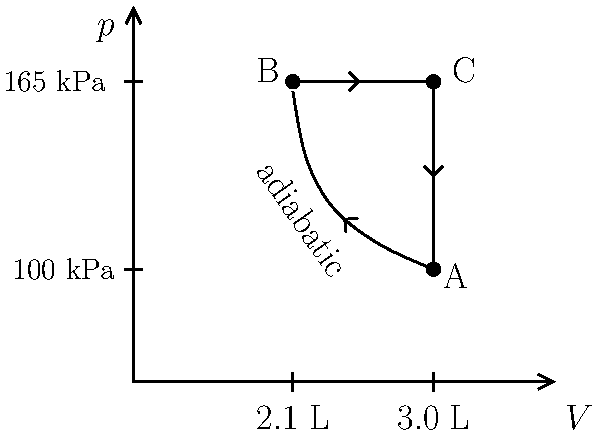
\includegraphics[width=2.5in]{gas_processes/pv_diagram.pdf}
\caption{For problem \ref{prob:chart}.}
\label{fig:pv_diagram}
\end{center}
\end{figure}
\medskip

\quad $A\to B$:  adiabatic compression
\medskip

\quad $B\to C$: constant pressure expansion
\medskip

\quad $C\to A$: cooling at constant volume
\medskip

Fill in the chart below for the change in thermal energy, heat flow
in, and work done \textit{on the gas} for each of the processes and for the
complete cycle.  {\bf Show all work.}

\[
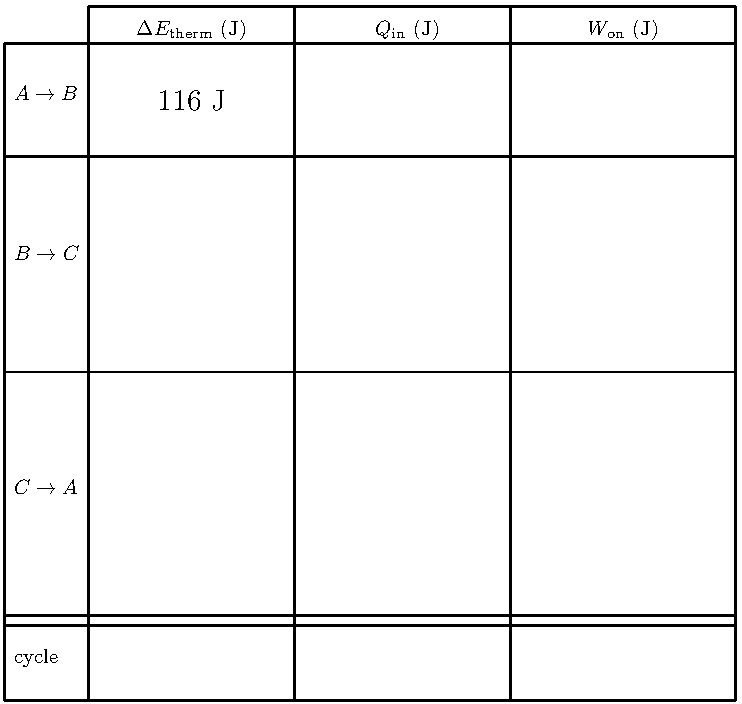
\includegraphics[width=3.5in]{gas_processes/chart.pdf}
\]
\label{prob:chart}
\end{problem}

\newpage

\begin{problem}
An amount $0.20$ moles of diatomic ideal gas undergoes the 
processes shown in the $p$-$V$ diagram (Fig.~\ref{fig:pv_processes}).
\begin{figure}
\begin{center}
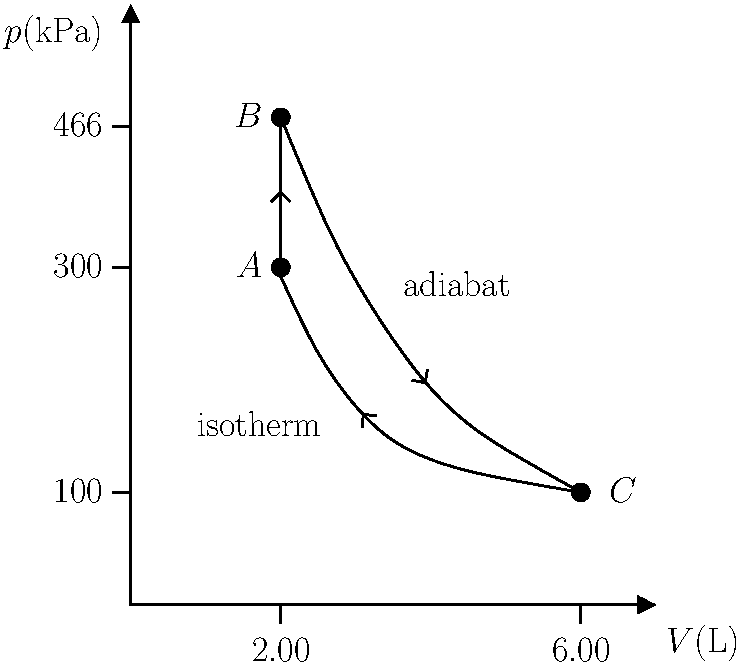
\includegraphics[width=2.5in]{gas_processes/pv_processes.pdf}
\caption{For problem \ref{prob:table}.}
\label{fig:pv_processes}
\end{center}
\end{figure}
\medskip
The table below has boxes for the change in thermal energy of the
gas, the heat added to the gas, and the work \textbf{done on} the gas,
all in joules. 
\smallskip
Energy values have already been entered in two of the
boxes. Fill in the remaining entries with values accurate to three
significant digits.  Be sure to show your work for each entry.

%\[
\begin{center}
\hspace{-1in}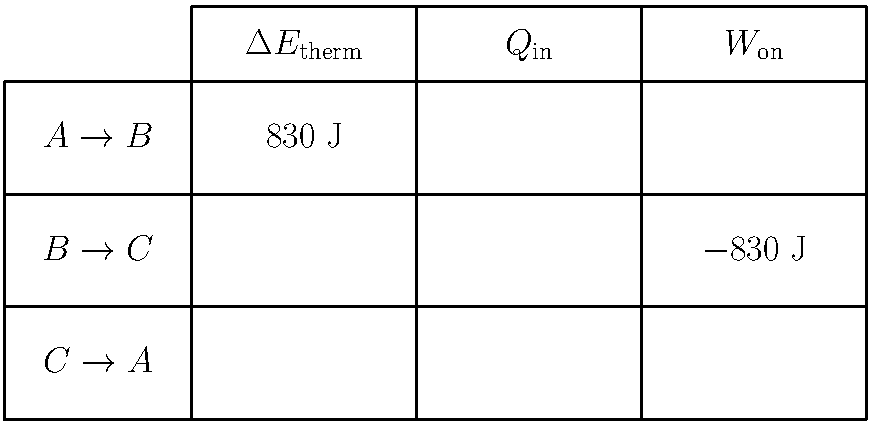
\includegraphics[width=4.5in]{gas_processes/table}
%\]
\end{center}
\label{prob:table}
\end{problem}

\begin{problem}
 The $pV$ diagram (Fig.~\ref{fig:from2011final}) shows a cyclic process for 2 moles 
 of an ideal monatomic gas.  
\begin{figure}
\begin{center}
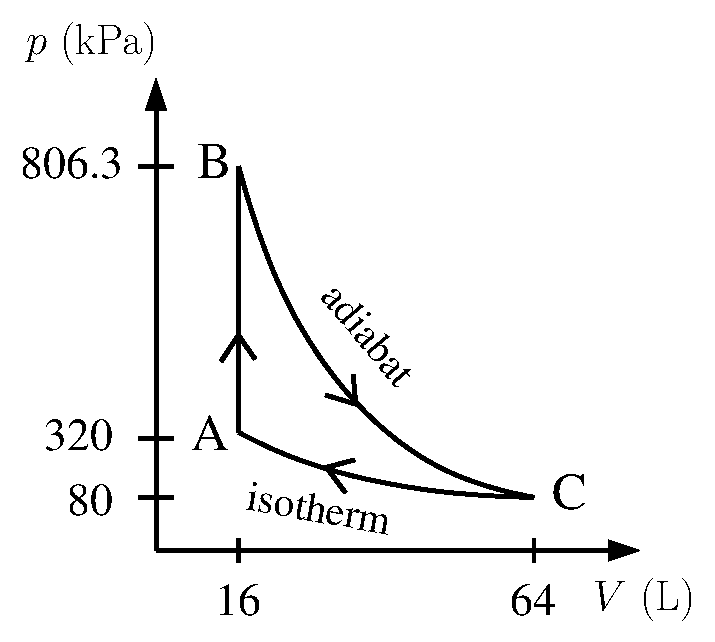
\includegraphics[width=2.5in]{gas_processes/pVfinal.eps}
\caption{For problem \ref{prob:from2011final}.}
\label{fig:from2011final}
\end{center}
\end{figure}

\begin{enumerate}
\item Determine the temperature of the gas at state {\bf A}.
\item Determine the heat flow into the gas during the process 
{\bf A}$\rightarrow${\bf B}.
\item Determine the heat flow into the gas during the process 
{\bf B}$\rightarrow${\bf C}.
\item Is the work done on the system for the complete cycle
positive, negative or zero? (No calculation required.)
\end{enumerate}
\label{prob:from2011final}
\end{problem}


%\begin{problem}
% By what factor must the volume of a gas with $\gamma = 1.4$ be
% changed in an adiabatic process if the kelvin temperature is to
% double?
%\label{prob:}
%\end{problem}

%\begin{problem}
% By how much does the temperature of (a) an ideal monatomic
% gas and (b) an ideal diatomic gas (with molecular rotation but no
% vibration) change in an adiabatic process in which $2.5\units{kJ}$ 
% of work id done on each mole of gas?
%\label{prob:}
%\end{problem}

%\begin{problem}
%An ideal gas expands to 10 times its original volume, main-
%taining a constant $440\units{K}$ temperature. If the gas does 
%$3.3\units{kJ}$ of work on its surroundings, (a) how much heat 
%does it absorb, and (b) how many moles of gas are there?
%\label{prob:}
%\end{problem}

%\begin{problem}
% A gas sample undergoes the cyclic process {\bf ABCA} shown in
% Fig. where {\bf AB} is an isotherm. The pressure at {\bf A} is 
% $60\units{kPa}$.  Find 
% \begin{enumerate}
% \item the pressure at {\bf B}, and 
% \item the net work done on the gas.
% \end{enumerate}
%\end{problem}


%\begin{problem}
%A $3.50\units{mol}$ sample of ideal gas with molar specific heat 
%$C = 5R/2$ is initially at a temperature $255\units{K}$  and 
%pressure $101\units{kPa}$. Determine the final
%temperature and the work done by the gas when $1.75\units{kJ}$ of heat
%are added to the gas 
%\begin{enumerate}
%\item isothermally, 
%\item at constant volume, and
%\item isobarically.
%\end{enumerate}
%\end{problem}

%\begin{problem}
%The curved path in Fig. lies on the $350\units{K}$ isotherm for an
%ideal gas with $\gamma = 1.4$
%\begin{enumerate}
%\item Calculate the net work done on the
%gas as it goes around the cyclic path {\bf ABCA}. 
%\item How much heat flows into or out of the gas on the 
%segment {\bf AB}?
%\end{enumerate}
%\label{prob:}
%\end{problem}

%\begin{problem}
%The curved path in Fig. lies on the $350\units{K}$ isotherm for an
%ideal gas with $\gamma = 1.4$
%\begin{enumerate}
%\item Calculate the net work done on the
%gas as it goes around the cyclic path {\bf ACDA}. 
%\item How much heat flows into or out of the gas on the 
%segment {\bf CD}?
%\end{enumerate}
%\label{prob:}
%\end{problem}



%\begin{problem}
%A $0.25\units{mol}$ sample of ideal gas initially occupies 
%$3.5\units{L}$. If it takes $61\units{J}$ of work to 
%compress the gas isothermally to $3.0\units{L}$, what's
%the temperature of the gas?
%\label{prob:}
%\end{problem}

%\begin{problem}
%A ideal gas sample undergoes the cyclic process {\bf ABCA} shown in
%Fig. , where {\bf AB} is an isotherm. The pressure at {\bf A} is 
%$60\units{kPa}$.
%Find 
%\begin{enumerate}
%\item the pressure at {\bf B}, and 
%\item the net work done on the gas.
%\end{enumerate}
%   \begin{figure}[h]
%   \begin{center}
%   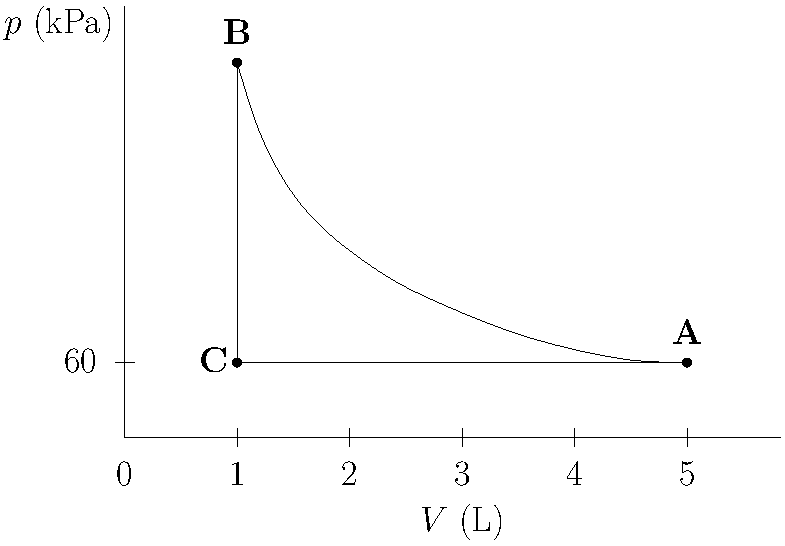
\includegraphics[width=3.0in]{gas_processes/cycle_w_isotherm_prob.pdf} 
%  \end{center} 
%   \caption{$p$-$V$ diagram for Problem \ref{prob:cycle_w_isotherm}}
%   \end{figure}
%\label{prob:cycle_w_isotherm}
%\end{problem}

%\begin{problem}
%An ideal gas with $\gamma = 1.4$ and $T = 300\units{K}$ starts at 
%point {\bf A} in Fig. It is   
%compressed adiabatically until its volume is $2.0\units{L}$ at {\bf B},
%and it is then cooled at constant pressure until it reaches $300\units{K}$
%at {\bf C}.  Finally it is allowed to expand isothermally back to 
%state {\bf A}.  Find 
%\begin{enumerate}
%\item the net work done on the gas, and 
%\item the minimum volume of the gas.
%\end{enumerate}
%\label{prob:}
%\end{problem}
%\newpage

%\begin{problem}
%A gas sample with the specific heat ratio $\gamma = 1.4$ undergoes 
%the cyclic process {\bf ABCA} shown in Fig. , where {\bf AB} is an adiabat. 
%The pressure at {\bf A} is $60\units{kPa}$.  Find 
%\begin{enumerate}
%\item the pressure at {\bf B}, and 
%\item the net work done on the gas.
%\end{enumerate}
%\begin{figure}[h]
%   \begin{center}
%   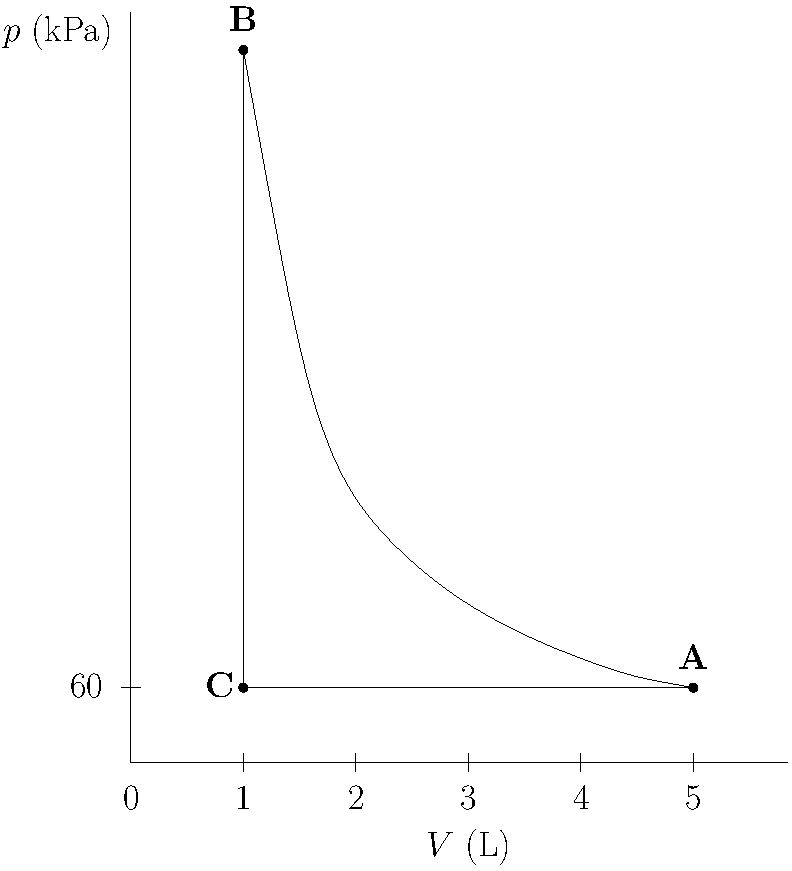
\includegraphics[width=2.5in]{gas_processes/cycle_w_adiabat_prob.pdf} 
%   \end{center} 
%   \caption{$p$-$V$ diagram for Problem \ref{prob:cycle_w_adiabat}}
%   \end{figure}
%\label{prob:cycle_w_adiabat}
%\end{problem}



